\documentclass[11pt]{scrartcl}
\usepackage{graphicx}
\graphicspath{{./}}
\usepackage[sexy]{evan}
\usepackage[normalem]{ulem}
\usepackage{hyperref}
\usepackage{mathtools}
\hypersetup{
    colorlinks=true,
    linkcolor=blue,
    filecolor=magenta,      
    urlcolor=cyan,
    pdfpagemode=FullScreen,
    }

\renewcommand{\dangle}{\measuredangle}

\renewcommand{\baselinestretch}{1.5}

\addtolength{\oddsidemargin}{-0.4in}
\addtolength{\evensidemargin}{-0.4in}
\addtolength{\textwidth}{0.8in}
% \addtolength{\topmargin}{-0.2in}
% \addtolength{\textheight}{1in} 


\setlength{\parindent}{0pt}

\usepackage{pgfplots}
\pgfplotsset{compat=1.15}
\usepackage{mathrsfs}
\usetikzlibrary{arrows}

\title{G3-4}
\author{Azzam Labib (IG: haxuv.world)}
\date{\today}
\begin{document}
\maketitle
\begin{enumerate}
    \item There are 14 children playing "The eagle catches the chicks." One of them is the 'eagle' while another child is the 'mother hen' whose job is to protect the 'chicks.' The rest of the children are the 'chicks.' After a while, the 'eagle' has caught 5 chicks. How many 'chicks' are still running around?
    \begin{enumerate}[label=(\alph*)]
        \item 6
        \item 7
        \item 8
        \item 9
        \item 10
    \end{enumerate}

    \item Find the number \( A \) such that the following statement is true: \( 7 \times A = 3 + 8 + 4 \times 8 \).
    \begin{enumerate}[label=(\alph*)]
        \item 3
        \item 4
        \item 5
        \item 7
        \item 8
    \end{enumerate}

    \item Two \$1 coins and ten 50¢ coins are randomly distributed among 4 children such that each child receives the same number of coins. What is the difference between the biggest amount and the smallest amount a child can receive?
    \begin{enumerate}[label=(\alph*)]
        \item 50¢
        \item \$1
        \item \$1.50
        \item \$2
        \item None of the above
    \end{enumerate}

    \item Tim is 8 years old and Sally is 4 years old. How old will Sally be when Tim is 14 years old?
    \begin{enumerate}[label=(\alph*)]
        \item 7 years old
        \item 8 years old
        \item 9 years old
        \item 10 years old
        \item None of the above
    \end{enumerate}

    \item Jane is 9 years old and John is 5 years old. How old will John be when Jane is 15 years old?
    
    \item A textbook is opened at random. To what pages is it opened if the product of the facing pages is 110?
    
    \item Find the number \( B \) such that the following statement is true: \( 8 \times B = 3 \times 9 + 5 \times 9 \).
    
    \item It is given that \( a \otimes b = a \times b + a - b \). For example, \( 2 \otimes 3 = 2 \times 3 + 2 - 3 \). Find the value of \( 4 \otimes 3 \).
    
    \item Jane has a rope of length 23 cm. She wants to cut the rope so that she can form the biggest possible square, where the length of each side, in cm, is a whole number. What is the length of the rope that she must cut to form the square?
    
    \item Find the missing term in the following sequence: 1, 2, 6, 24, \_\_\_\_, 720.
    
    \item On National Day, 39 soldiers lined up in a straight row on opposite sides of Stadium Street to welcome Prime Minister Lee. A soldier stands on each end of Stadium Street. The distance between two adjacent soldiers on either side was 20 m. The soldiers on one side were arranged such that each soldier filled the gap between two other soldiers on the opposite side. How long was Stadium Street?
    
    \item A shop sells sweets where every 3 sweet wrappers can be exchanged for one more sweet. Sharon has enough money to buy only 11 sweets. What is the biggest number of sweets that she can get from the shop?
    
    \item At a workshop, there are 10 participants. Each of them shakes hand once with one another. How many handshakes are there?
    
    \item Ali uses identical square tiles to make the following figures. If he continues using the same pattern, how many tiles will there be in the 15th figure?
    \begin{figure}[h]
        \centering
        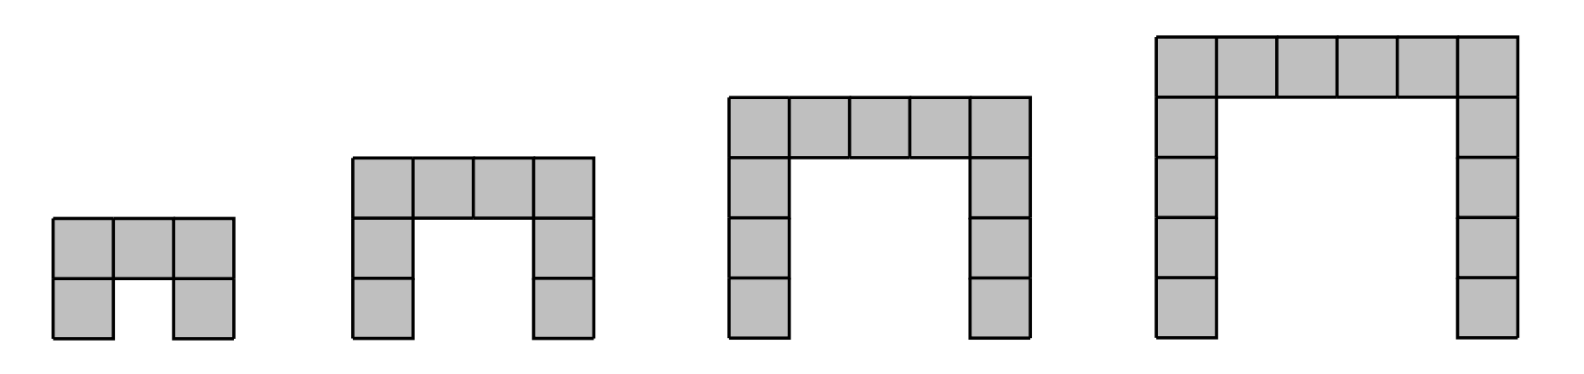
\includegraphics[width=0.5\textwidth]{StarGen/G7-8 and G3-4/diagram.png}
    \end{figure}
    
    \item What is the least number of cuts required to cut 16 identical sausages so that they can be shared equally among 24 people?
    
    \item A vending machine accepts 10¢ coins, 20¢ coins, 50¢ coins, and \$1 coins only. Ivy wants to buy a can of drink that costs \$1.60. She has eight 10¢ coins, three 20¢ coins, two 50¢ coins and one \$1 coin. If she wants to get rid of as many coins as possible without the combination of coins that she should use in the vending machine?

       \item The total cost of a pen and a pencil is \$2.90. The pen costs 60¢ more than the pencil. What much does the pen cost?
    
    \item If the three-digit number 3N3 is divided by 9, the remainder is 1. Find \( N \).
    
    \item Charles has 16 marbles. He divides them into 4 piles so that each pile has a different number of marbles. Find the smallest possible number of marbles in the biggest pile.

    \item In the following alphametic, all the different letters stand for different digits. Find the three-digit sum SEE.
    \begin{figure}[h]
        \centering
        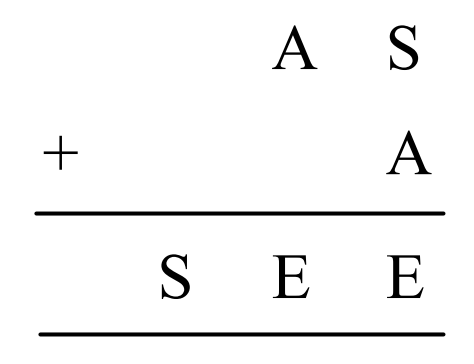
\includegraphics[width=0.3\textwidth]{StarGen/G7-8 and G3-4/see.png}
    \end{figure}
    
    \item A teacher has a bag of sweets to treat her class. If she gave 5 sweets to each student, then she would have 40 sweets left. If she gave 7 sweets to each student, then she would have 6 sweets left. How many students and how many sweets are there?
    
    \item What are the last 2 digits of the sum \( 1 + 11 + 111 + \ldots + 111\ldots111 \)? (50 digits in the last term)
    
    \item Alvin tells the truth on Monday, Tuesday, Wednesday, and Thursday. He lies on all other days. Doris tells the truth on Monday, Friday, Saturday, and Sunday. She lies on all other days. One day they both said, "Yesterday I lied." When was that one day?

        
    \item Find the total number of triangles in the diagram.
    \begin{figure}[h]
        \centering
        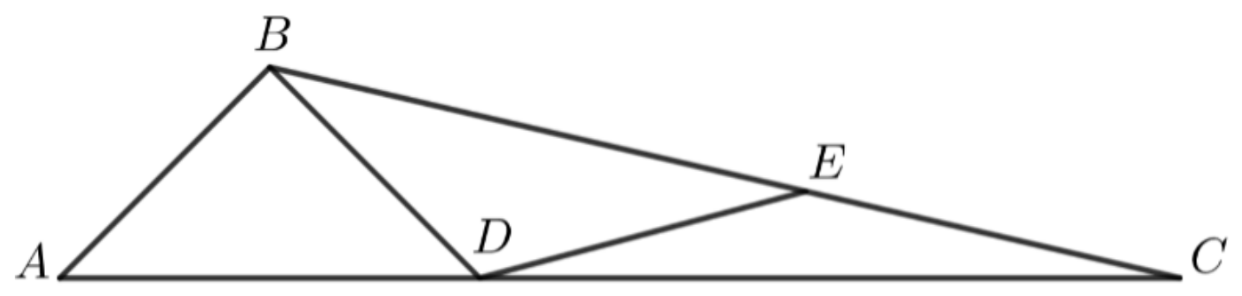
\includegraphics[width=0.3\textwidth]{StarGen/G7-8 and G3-4/triangle.png}
    \end{figure}
\end{enumerate}
\end{document}